\documentclass{beamer}

\usepackage{graphicx}
\usepackage{physics}
\usepackage{amsmath}
\usepackage{tikz}
\usepackage{polyglossia}
\usepackage{booktabs}
\setdefaultlanguage{english}
\usepackage[backend=biber,style=authortitle]{biblatex}

\usetikzlibrary{shapes.geometric,decorations.pathmorphing,patterns,calc}

\addbibresource{biblio.bib}

\beamertemplatenavigationsymbolsempty

\renewcommand{\arraystretch}{2}

\begin{document}
\title{Wireless Power Transfer by\\Resonant Inductive Coupling}
\author{Isawan Millican}
\institute{
  School of Physics and Astronomy\\
  University of Nottingham
  }
\subject{Physics}
\frame{\titlepage}
\begin{frame}
  \frametitle{Contents}
\tableofcontents
\end{frame}

\section{Types of wireless power transfer}
\begin{frame}
  \frametitle{Types of wireless power transfer}
  Wireless power transfer can be broadly grouped depending on the effective range.
  \begin{table}
    \begin{tabular*}{.75\textwidth}{@{\extracolsep{\fill}} c c}
      \toprule
      \textbf{Near-field} & \textbf{Far-Field} \\\hline
      Inductive coupling  & Microwaves \\
      Capacitive coupling  & Lasers \\ \bottomrule
    \end{tabular*}
    \caption{Types of wireless power transfer scheme}
  \end{table}
\end{frame}


\section{Review of Electromagnetic Induction}
\begin{frame}
  \frametitle{Review of Electromagnetic Induction}
  \begin{figure}
      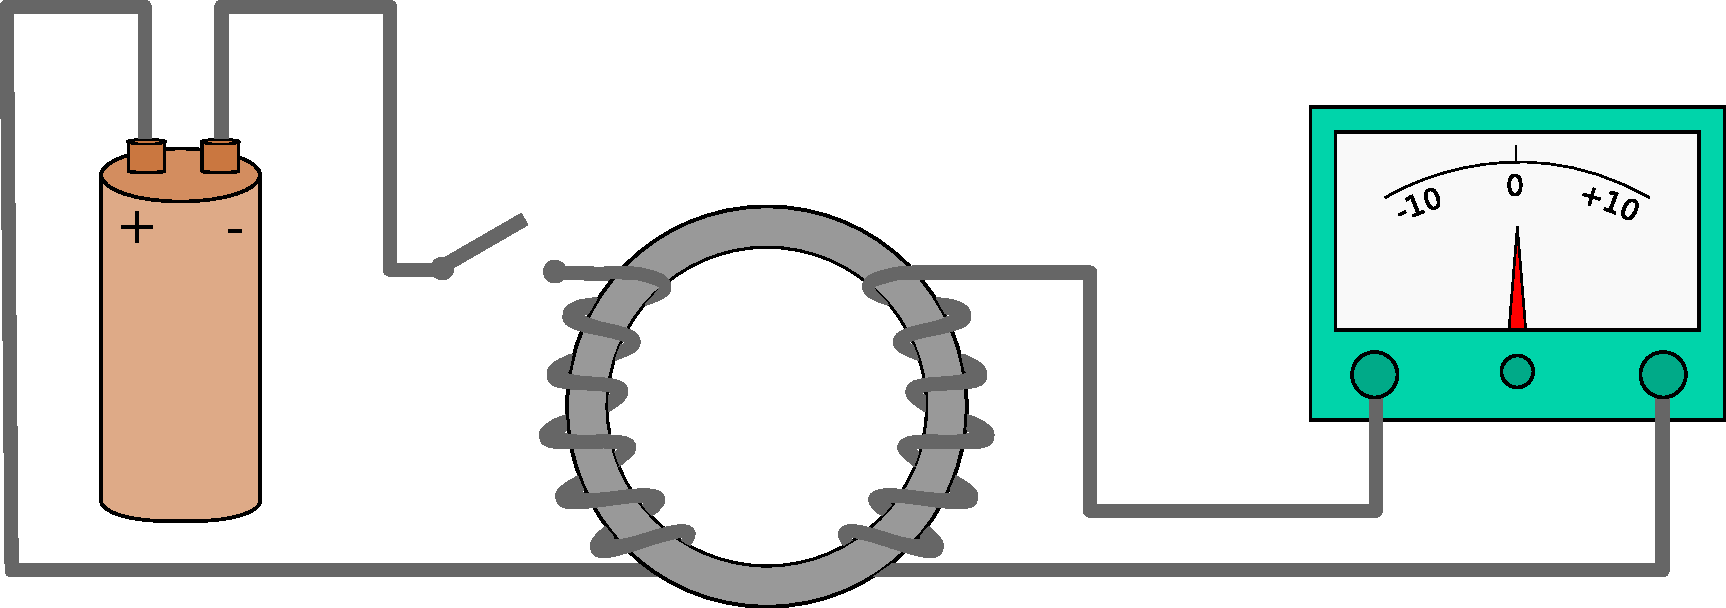
\includegraphics[scale=0.3]{images/faraday.pdf}
      \caption{Diagram of Faraday's apparatus.
      Changes in the magnetic field of the left coil induces a current in the right coil.
      \textcite{hyperphysicsresonate}}
  \end{figure}
  Faraday showed in 1831, magnetic fields.
\end{frame}


\section{Wireless power transfer}
\begin{frame}
  \frametitle{Wireless power transfer}
  \begin{figure}
    %\usetikzlibrary{shapes.geometric,decorations.pathmorphing,patterns,calc}

\begin{tikzpicture}[square/.style={regular polygon,regular polygon sides=4}]


% Oscillator
\node (oscillator) at (1,.25) [square,draw, minimum width=15mm,fill=lightgray]
{\tikz \draw[scale=0.07,domain=-3.141:3.141,smooth,variable=\t] plot (\t,{sin(\t r)});};
\coordinate (pcoila) at ($ (oscillator) + (-.3,2)$);
\coordinate (pcoilb) at ($ (oscillator) + (.3,2)$);
\node[circle,fill=black,inner sep=.5mm] (a) at ($(oscillator) + (-1,-0.25)$) {};
\node[circle,fill=black,inner sep=.5mm] (b) at ($(oscillator) + (-1,0.25)$) {};
\draw (a) -- (oscillator.west |- a);
\draw (b) -- (oscillator.west |- b);
\draw[decoration={aspect=0.2,segment length=1.6mm, amplitude=5mm,coil},decorate] (pcoila) -- (pcoilb);
\draw (pcoila) -- (pcoila |- oscillator.north);
\draw (pcoilb) -- (pcoilb |- oscillator.north);

% Rectifier
\node (rectifier) at (5,.25) [square,draw,minimum width=15mm,fill=lightgray] {};
\coordinate (scoila) at ($ (rectifier) + (-.3,2)$);
\coordinate (scoilb) at ($ (rectifier) + (.3,2)$);
\node[circle,fill=black,inner sep=.5mm] (c) at ($(rectifier) + (1,-0.25)$) {};
\node[circle,fill=black,inner sep=.5mm] (d) at ($(rectifier) + (1,0.25)$) {};
\draw (c) -- (rectifier.east |- c);
\draw (d) -- (rectifier.east |- d);
\draw[decoration={aspect=0.2,segment length=1.6mm, amplitude=5mm,coil},decorate] (scoila) -- (scoilb);
\draw (scoila) -- (scoila |- rectifier.north);
\draw (scoilb) -- (scoilb |- rectifier.north);
% Rectifier symbol
\coordinate (ra) at ($(rectifier)+(0,-0.2)$);
\coordinate (rb) at ($(rectifier)+(-.25,.2)$);
\coordinate (rc) at ($(rectifier)+(.25,.2)$);
\coordinate (ral) at ($(ra)+(.2,0)$);
\coordinate (rar) at ($(ra)+(-.2,0)$);
\draw (rar)--(ra)--(ral);
\draw[fill=black] (ra)--(rb)--(rc) -- cycle;

% Labels
\node at (oscillator) [below=20] {Oscillator};
\node at (oscillator) [left=30] {Power in};
\node at (rectifier) [below=20] {Rectifier};
\node at (rectifier) [right=30] {Power out};
\end{tikzpicture}

    \caption{A simple induction apparatus to transmit power wirelessly.}
  \end{figure}
  \begin{itemize}
    \item Remove the iron core.
    \item Magnetic flux through coil is low due to field divergence.
    \item Efficient only if coils are adjacent.
    \item Range can be extended with resonance.
  \end{itemize}
\end{frame}


\section{Resonant circuit}
\begin{frame}
  \frametitle{Resonant circuit}
  \begin{itemize}
    \item A resonant circuit has a strong response to an oscillating voltage
      with frequency $\omega_0$
    \item In the induction system, the voltage is induced by a magnetic field.
  \end{itemize}
  \begin{figure}
  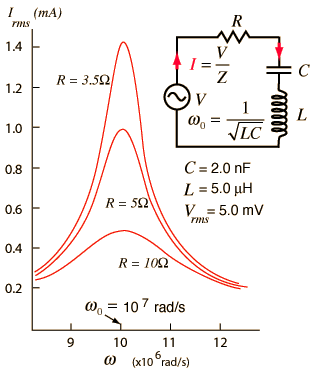
\includegraphics[scale=0.3]{images/RLC.png}
  \caption{An RLC circuit
    and its response to a driving oscillating voltage.
    \textcite{hyperphysicsresonate}}
  \end{figure}
\end{frame}

\section{Resonant inductive coupling}
\begin{frame}
  \frametitle{Resonant inductive coupling}
  \begin{itemize}
    \item The resonant responses strongly couples the RLC circuits.
    \item Highly efficient for distances within one wavelength.
  \end{itemize}
  \begin{figure}
    \usetikzlibrary{shapes.geometric,decorations.pathmorphing,patterns,calc}

\begin{tikzpicture}[square/.style={regular polygon,regular polygon sides=4}]

% Oscillator
\node (oscillator) at (1,.25) [square,draw, minimum width=15mm,fill=lightgray]
{\tikz \draw[scale=0.07,domain=-3.141:3.141,smooth,variable=\t] plot (\t,{sin(\t r)});};
\coordinate (pcoila) at ($ (oscillator) + (-.3,2)$);
\coordinate (pcoilb) at ($ (oscillator) + (.3,2)$);
\node[circle,fill=black,inner sep=.5mm] (a) at ($(oscillator) + (-1,-0.25)$) {};
\node[circle,fill=black,inner sep=.5mm] (b) at ($(oscillator) + (-1,0.25)$) {};
\draw (a) -- (oscillator.west |- a);
\draw (b) -- (oscillator.west |- b);
\draw[decoration={aspect=0.2,segment length=1.6mm, amplitude=5mm,coil},decorate] (pcoila) -- (pcoilb);
\draw (pcoila) -- (pcoila |- oscillator.north);
\draw (pcoilb) -- (pcoilb |- oscillator.north);


% Rectifier
\node (rectifier) at (5,.25) [square,draw,minimum width=15mm,fill=lightgray] {};
\coordinate (scoila) at ($ (rectifier) + (-.3,2)$);
\coordinate (scoilb) at ($ (rectifier) + (.3,2)$);
\node[circle,fill=black,inner sep=.5mm] (c) at ($(rectifier) + (1,-0.25)$) {};
\node[circle,fill=black,inner sep=.5mm] (d) at ($(rectifier) + (1,0.25)$) {};
\draw (c) -- (rectifier.east |- c);
\draw (d) -- (rectifier.east |- d);
\draw[decoration={aspect=0.2,segment length=1.6mm, amplitude=5mm,coil},decorate] (scoila) -- (scoilb);
\draw (scoila) -- (scoila |- rectifier.north);
\draw (scoilb) -- (scoilb |- rectifier.north);
% Rectifier symbol
\coordinate (ra) at ($(rectifier)+(0,-0.2)$);
\coordinate (rb) at ($(rectifier)+(-.25,.2)$);
\coordinate (rc) at ($(rectifier)+(.25,.2)$);
\coordinate (ral) at ($(ra)+(.2,0)$);
\coordinate (rar) at ($(ra)+(-.2,0)$);
\draw (rar)--(ra)--(ral);
\draw[fill=black] (ra)--(rb)--(rc) -- cycle;


% Primary resonator
\coordinate (pcap) at (2,1.25);
\coordinate (pcapa) at ($(pcap)+(-.05,0)$);
\coordinate (pcapb) at ($(pcap)+(.05,0)$);
\coordinate (pcapcoila) at ($ (pcap) + (-.3,1)$) [circle,draw] {};
\coordinate (pcapcoilb) at ($ (pcap) + (.3,1)$) [circle,draw] {};
\draw[decoration={aspect=.2,segment length=1.6mm,amplitude=5mm,coil},decorate] (pcapcoila) -- (pcapcoilb);
\draw (pcapa) -| (pcapcoila);
\draw (pcapb) -| (pcapcoilb);
\draw[thick] ($(pcapa) +(0,.2)$) -- ($(pcapa) +(0,-.2)$);
\draw[thick] ($(pcapb) +(0,.2)$) -- ($(pcapb) +(0,-.2)$);


% Secondary resonator
\coordinate (scap) at (4,1.25);
\coordinate (scapa) at ($(scap)+(-.05,0)$);
\coordinate (scapb) at ($(scap)+(.05,0)$);
\coordinate (scapcoila) at ($ (scap) + (-.3,1)$) [circle,draw] {};
\coordinate (scapcoilb) at ($ (scap) + (.3,1)$) [circle,draw] {};
\draw[decoration={aspect=.2,segment length=1.6mm,amplitude=5mm,coil},decorate] (scapcoila) -- (scapcoilb);
\draw (scapa) -| (scapcoila);
\draw (scapb) -| (scapcoilb);
\draw[thick] ($(scapa) +(0,.2)$) -- ($(scapa) +(0,-.2)$);
\draw[thick] ($(scapb) +(0,.2)$) -- ($(scapb) +(0,-.2)$);

% Magnetic field
\coordinate (fau) at ($(pcoila) + (-.5,.5)$);
\coordinate (fad) at ($(pcoila) + (-.5,-.5)$);
\coordinate (fbu) at ($(scoilb) + (.5,.5)$);
\coordinate (fbd) at ($(scoilb) + (.5,-.5)$);
\draw [blue] plot [smooth] coordinates {(fau) ($(pcoilb)+(0,.25)$)
                                              ($(pcapcoilb)!.5!(scapcoila)+(0,.5)$)
                                              ($(scoila)+(0,.25)$)
                                              (fbu) };
\draw [blue] plot [smooth] coordinates {(fad) ($(pcoilb)+(0,-.25)$)
                                              ($(pcapcoilb)!.5!(scapcoila)+(0,-.5)$)
                                              ($(scoila)+(0,-.25)$)
                                              (fbd) };

% Labels
\node at (oscillator) [below=20] {Oscillator};
\node at (oscillator) [left=30] {Power in};
\node at (rectifier) [below=20] {Rectifier};
\node at (rectifier) [right=30] {Power out};
\node (labelreso) at ($ (pcap)!.5!(scap) $) [below=7mm] {Resonant circuits};
\path (labelreso) edge[->,thick] ($(pcap)!.25!(labelreso)$);
\path (labelreso) edge[->,thick] ($(scap)!.25!(labelreso)$);

\end{tikzpicture}


    \caption{The divergence of the magnetic field is reduced by the addition
    of an RLC resonant circuit.}
  \end{figure}
\end{frame}

\section{Efficiency}
\begin{frame}
  \frametitle{Efficiency}
  Theoretical analysis shows for a distance of 5 times greater than the coil radius,
  the efficiency of the system is 52\%\footcite{Efficient}.
\end{frame}

\section{Applications}
\begin{frame}
  \frametitle{Applications: Smartcard}
  \begin{figure}
    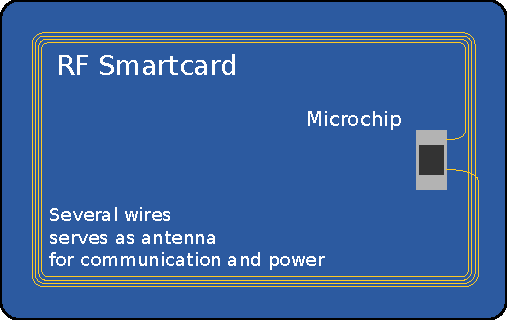
\includegraphics[scale=0.75]{images/smartcard.pdf}
    \caption{A diagram of a smartcard. \textcite{wikiRIC}}
  \end{figure}
\end{frame}
\begin{frame}
  \center
  \begin{block}{Any questions?}
  \end{block}
\end{frame}

\end{document}
